\documentclass[10pt]{extarticle}

% Lingua e matematica
\usepackage[english]{babel}
\usepackage{amsmath,amssymb,amsthm}

% Grafica e tabelle
\usepackage{graphicx}
\usepackage{subcaption}
\usepackage{float}
\usepackage{booktabs}
\usepackage{multirow}
\usepackage{siunitx}
\usepackage{wrapfig}
\usepackage{placeins}


% Codice (opzionale)
\usepackage{listings}
\usepackage{xcolor}
\definecolor{codegreen}{rgb}{0,0.6,0}
\definecolor{codegray}{rgb}{0.5,0.5,0.5}
\definecolor{codepurple}{rgb}{0.58,0,0.82}
\definecolor{backcolour}{rgb}{0.98,0.98,0.98}
\lstdefinestyle{mystyle}{
  backgroundcolor=\color{backcolour},
  commentstyle=\color{codegreen},
  keywordstyle=\color{magenta},
  numberstyle=\tiny\color{codegray},
  stringstyle=\color{codepurple},
  basicstyle=\ttfamily\footnotesize,
  breaklines=true, keepspaces=true, numbers=none, tabsize=2
}
\lstset{style=mystyle}

% Margini
\usepackage[margin=0.6in]{geometry}
\usepackage{ragged2e}
\usepackage{enumitem}
%\usepackage[utf8]{inputenc} % per caratteri UTF-8 nei .tex e nel .bib
\usepackage[backend=biber,style=ieee,sorting=none,maxbibnames=99]{biblatex}
\ExecuteBibliographyOptions{doi=true,url=true,isbn=false}
\addbibresource{references.bib}
\usepackage{csquotes}       % consigliato da biblatex (evita warning e parse strani)
\usepackage{pifont}
\newcommand{\good}[1]{\textcolor{teal!70!black}{\ding{51}~#1}}



% Bibliografia (biblatex + biber)
\usepackage[backend=biber,style=ieee]{biblatex}
\addbibresource{references.bib}

% TOC: includi anche \paragraph e numerali
\setcounter{secnumdepth}{2}
\setcounter{tocdepth}{2}

% Hyperref (sempre *dopo* gli altri pacchetti)
\usepackage[colorlinks=true,linkcolor=blue,citecolor=teal,urlcolor=magenta]{hyperref}


\begin{document}

% Custom header without a separate titlepage
\noindent
\begin{minipage}{0.3\textwidth}
    
\includegraphics[width=1.3\linewidth]{Figures/polito_logo_2021_blu.jpg}
\end{minipage}
\hfill
\begin{minipage}{0.68\textwidth}
    \raggedleft
    {\LARGE \textbf{Politecnico di Torino}}\\[0.2cm]
    {\large Master's Degree in Mathematical Engineering}\\[0.7cm]
    {\large \textbf{Material for Thesis}}\\[0.2cm]
    {\large c-- Data Pre-processing Pipeline \\ Intra and Inter Analysis}\\[0.7cm]
    \begin{tabular}{rl}
        Elisabetta Roviera & \texttt{s328422} \\
    \end{tabular}
\end{minipage}

\vspace{1cm}
\hrule
\vspace{0.5cm}

\tableofcontents

\vspace{0.5cm}
\hrule
\vspace{1cm}


% Main content begins here, on the same page
\justifying

\begin{abstract}
{\color{red}
\textbf{MANCA L'ABSTRACT.}
}
\end{abstract}

\section{Intra-Dataset Pre-processing}
\label{sec:intra_preprocessing}
Data pre-processing represents a foundational stage in DNA methylation analysis, particularly in cancer epigenomics,
where technical artefacts, probe-design biases, and unwanted sources of variation can obscure or distort genuine
biological signals. Before performing feature selection, or machine-learning models, it is essential
to ensure that the methylation matrices used for statistical modelling are accurate, harmonised across platforms, and free
from unreliable probes or batch-associated effects.

In the context of breast cancer, where early epigenetic alterations may be subtle and highly localized, careful
pre-processing is crucial to avoid confounding Normal–Adjacent differences with technical noise. Several well-established
sources of unreliability—cross-reactive probes, SNP-affected loci, non-CpG targets, Infinium Type~I/II probe-design
bias, and batch effects—must be addressed through a systematic and reproducible workflow.  

The primary goal of this section is therefore to construct, for each dataset, a high-quality and biologically coherent
methylation matrix suitable for downstream analyses. To this end, all datasets undergo the same structured pipeline:
initial alignment and quality checks; removal of unreliable CpGs through literature-based technical filtering; identification of invariant CpGs that
carry no discriminative information along the Normal–Adjacent axis; conversion
from $\beta$-values to M-values for statistical modelling; and correction of batch effects.

These steps ensure methodological consistency across the three cohorts (GSE69914 [\ref{subsec:gse69914_preproc}], GSE225845 [\ref{subsec:gse225845_preproc}], GSE287331 [\ref{subsec:gse287331_preproc}]) and
provide a unified, denoised, and biologically meaningful set of features to be used in the subsequent analyses of early
epigenetic alterations.


% ============================================================
\subsection{Dataset GSE69914}
\label{subsec:gse69914_preproc}
% ============================================================

\paragraph{Step~0 -- Initial Pre-processing}
\label{par:gse69914_step0}

The initial pre-processing stage verifies the structural integrity of the dataset.
The $\beta$-value matrix and its corresponding phenotype table were imported from
their Parquet representations. Both tables contained \good{397 samples}, and the $\beta$-matrix included
\good{485{,}512 CpGs}, confirming full dataset availability at load time.

Sample identifiers in the phenotype table were inspected to ensure uniqueness and correct metadata structure. No
duplicated \texttt{id\_tissue} entries were detected \good{(0 duplicates)}, and all required fields (\texttt{id\_tissue}, \texttt{label})
were present \good{(0 missing fields)}, indicating that the phenotype annotation is complete and coherent. Alignment
between the phenotype table and the $\beta$-matrix was assessed by intersecting sample IDs. All samples were shared
across matrices, yielding \good{perfect correspondence (397/397 matched)}.

A probe-level and sample-level missingness check was then performed to verify the completeness of the methylation
matrix. The entire dataset was found to be fully observed, with \good{0 missing CpG values} and \good{0 missing sample
entries}. This confirms that no early NaN filtering or imputation is required for this dataset.

\paragraph{Step~1 -- Infinium Type I/II Bias Diagnostics}
\label{subpar:gse69914_typebias}

\begin{figure}[t]
    \centering
    \begin{subfigure}[t]{0.49\textwidth}
        \centering
        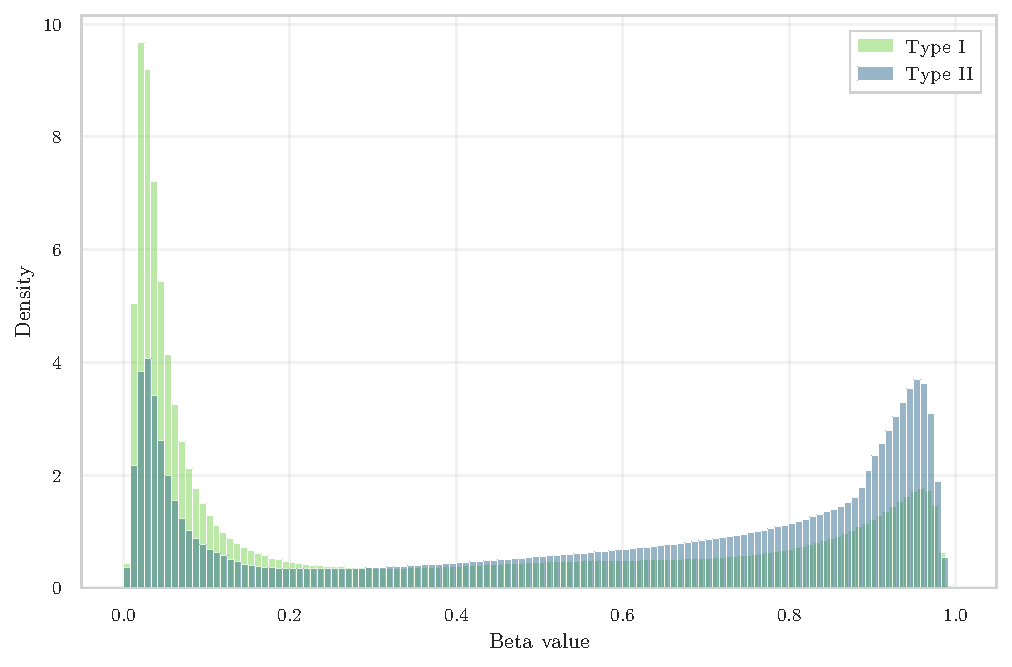
\includegraphics[height=6cm]{Figures/GSE69914_type_bias_density.pdf}
        \caption{$\beta$-value distribution by Infinium probe design (Type~I vs.~Type~II). 
        The near-overlapping shapes indicate effective correction of probe-type bias.}
        \label{fig:type_bias_density}
    \end{subfigure}
    \hfill
    \begin{subfigure}[t]{0.49\textwidth}
        \centering
        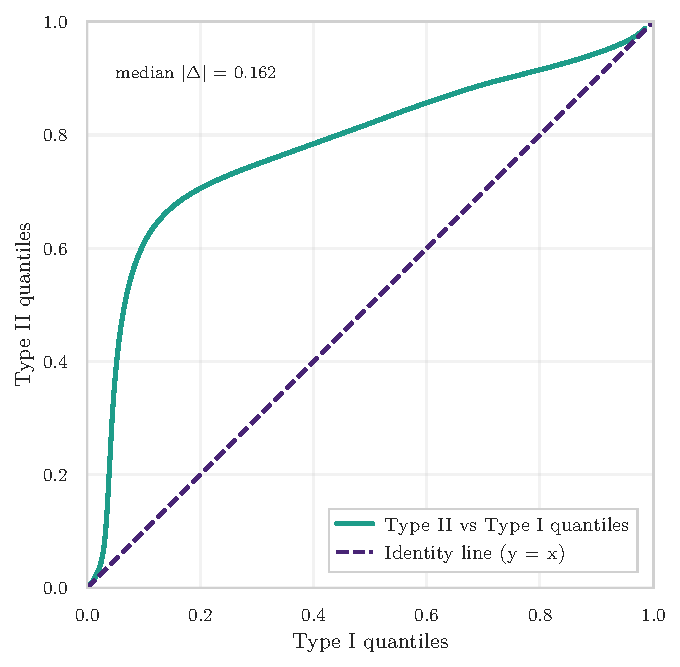
\includegraphics[height=6cm]{Figures/GSE69914_type_bias_qqplot.pdf}
        \caption{Q--Q plot comparing quantiles of Type~II vs.~Type~I probes. 
        The alignment to the diagonal ($y = x$) confirms balanced signal distributions after normalization.}
        \label{fig:type_bias_qq}
    \end{subfigure}
    \caption{Diagnostic evaluation of Infinium Type~I/II probe bias correction in the GSE69914 dataset. 
    The consistent $\beta$-value and quantile distributions demonstrate the effectiveness of the BMIQ normalization previously applied.}
    \label{fig:type_bias_combined}
\end{figure}

Raw methylation intensity data (\textit{IDAT} files) were processed by the original authors using the
\texttt{minfi} pipeline and \texttt{BMIQ} normalization, as reported in \cite{GSE69914}.  
A well-known characteristic of Illumina Infinium microarrays is the \textbf{systematic technical bias between
Type~I and Type~II probes}.  
This bias has been extensively documented in the literature, most notably by Maksimovic
\textit{et al.}~\cite{Maksimovic2012SWAN}, who showed that the two probe chemistries produce inherently different
$\beta$-value distributions and therefore require appropriate probe-type normalization.  
Such differences, if uncorrected, can propagate into downstream statistical analyses.

To independently verify that this bias had been successfully mitigated in the present dataset, $\beta$-values were
stratified by probe design (Type~I vs.~Type~II) using the official Illumina 450K manifest
from Bioconductor~\cite{Illumina450kAnno}.  
Following the diagnostic procedure of Teschendorff \textit{et al.}~\cite{Teschendorff2013BMIQ}, two complementary
assessments were performed:

\begin{enumerate}
    \item \textbf{Density comparison.}  
    As shown in Fig.~\ref{fig:type_bias_density}, the $\beta$-value distributions of Type~I and Type~II probes
    substantially overlap, indicating the absence of the multi-modal distortion typical of unnormalized data.
    \item \textbf{Quantile--quantile alignment.}  
    The Q--Q plot in Fig.~\ref{fig:type_bias_qq} exhibits quite a diagonal trend for Type~II vs.~Type~I
    quantiles, which is the expected signature of balanced probe-type scaling after normalization.
\end{enumerate}

The resulting pattern closely matches the characteristic behaviour described by Teschendorff
\textit{et al.}~\cite{Teschendorff2013BMIQ} and Wang \textit{et al.}~\cite{Wang2015Normalization450K}, while being fully
consistent with the probe-type discrepancies originally analysed by Maksimovic \textit{et al.}~\cite{Maksimovic2012}.  
\good{Together, these diagnostics confirm that the dataset has undergone effective Type~I/II probe bias correction.}



\paragraph{Step~2 -- Technical Filtering}
\label{par:gse69914_step2}

\begin{figure}[t]
    \centering

    % Panel (a)
    \begin{subfigure}[t]{0.48\textwidth}
        \centering
        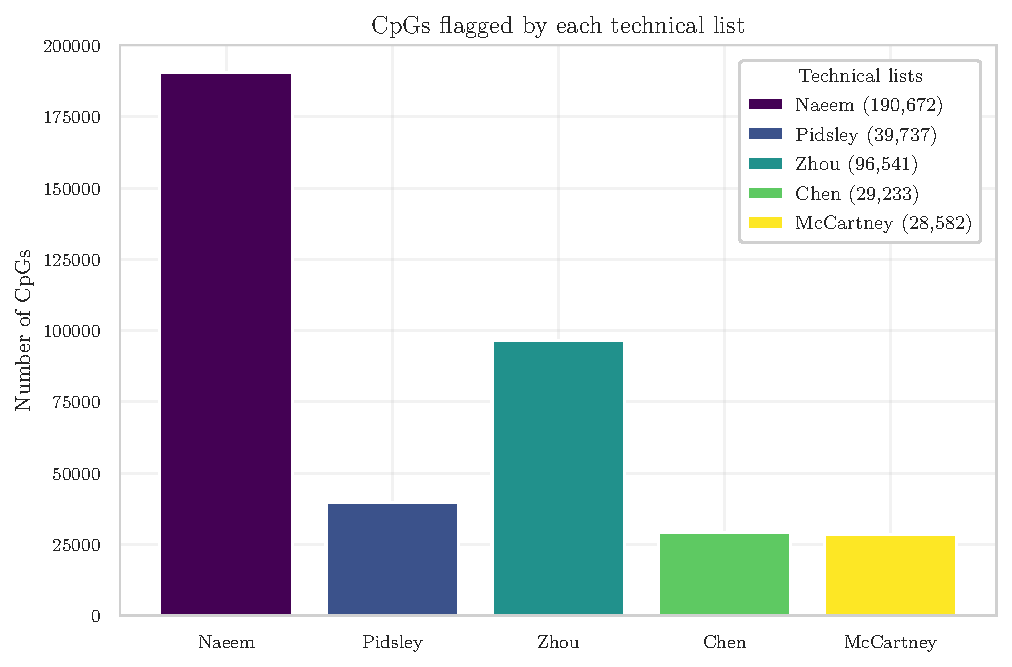
\includegraphics[width=\textwidth]{Figures/GSE69914_technical_lists_barplot.pdf}
        \caption{
            CpGs flagged by each technical filtering resource 
            (Naeem, Pidsley, Zhou \texttt{MASK\_*}, Chen, McCartney). 
        }
        \label{fig:gse69914_tech_barplot}
    \end{subfigure}
    \hfill
    % Panel (b)
    \begin{subfigure}[t]{0.48\textwidth}
        \centering
        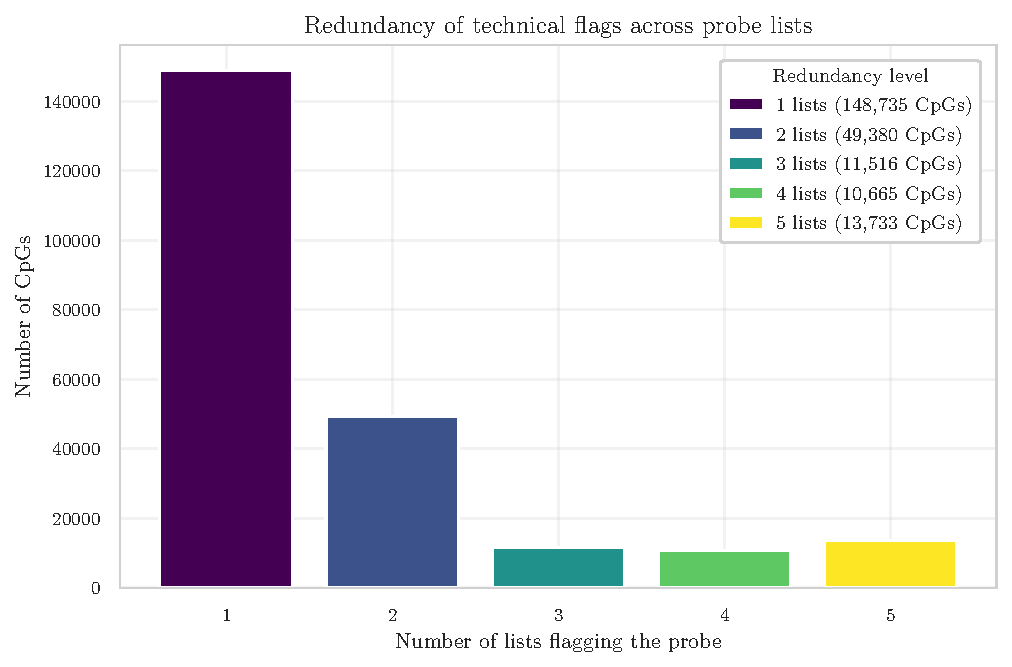
\includegraphics[width=\textwidth]{Figures/GSE69914_technical_lists_redundancy_histogram.pdf}
        \caption{
            Redundancy distribution of probes flagged by 1--5 lists. 
        }
        \label{fig:gse69914_tech_redundancy}
    \end{subfigure}

    \caption{
        Summary of technical filtering for the GSE69914 methylation dataset. 
        \textbf{(a)} Intersection between the dataset and each external probe-filtering resource, 
        showing the number of CpGs flagged by Naeem, Pidsley, Zhou, Chen, and McCartney lists. 
        \textbf{(b)} Redundancy analysis indicating how many probes were simultaneously flagged 
        by 1 to 5 independent resources, quantifying the concordance among technical annotations.
    }
    \label{fig:gse69914_technical_filtering}
\end{figure}


Technical filtering aims to remove unreliable or biologically confounded probes prior to statistical modelling.  
This stage reduces noise, improves downstream reproducibility, and ensures that only high-confidence CpG loci are
retained for analysis (Fig.~\ref{fig:gse69914_technical_filtering}).

\subparagraph{Exclusion of technical probe sets}
A collection of curated probe resources was used to exclude loci known to exhibit technical artefacts  
(see Appendix~\ref{app:probe-filters} for details).  
These include probes affected by common genetic variants at the CpG or single-base extension site
\cite{zhou2016,pidsley2016}, probes with demonstrated multi-mapping or off-target hybridisation  
\cite{chen2013,mccartney2016}, and probes flagged by the \texttt{MASK\_*} reliability annotations  
\cite{zhou2016}.  
Additional quality control criteria follow the hierarchical filtering strategy of Naeem et al.\ \cite{naeem2014},
which targets multi-mapping loci, repeat structures, and disruptive SNPs.

The overlaps between these resources and the $\beta$-matrix were substantial  
(Fig.~\ref{fig:gse69914_tech_barplot}).  
A total of \good{190{,}672 probes} were flagged by Naeem et al., \good{39{,}737} by Pidsley et al.,
\good{29{,}233} by Chen et al., \good{96{,}541} by the Zhou \texttt{MASK\_*} fields, and
\good{28{,}582} by McCartney et al.\  
These lists are known to partially overlap—particularly those focused on multi-mapping and SNP-associated
unreliability—and their union resulted in the removal of \good{225{,}426 unique CpGs}.  
After this operation, \good{260{,}086 CpGs} remained.

\subparagraph{Annotation-based filtering (Illumina manifest)}
\label{subpar:gse69914_noncpg}

To ensure consistency with the manufacturer’s official annotation, the HumanMethylation450 v1.2 manifest \cite{Illumina450kManifest} was used to
validate probe identity and genomic mapping.  
Through this annotation, probes lacking valid chromosome information, those with undefined genomic coordinates, and
those targeting non-CpG contexts (IDs beginning with ``\texttt{ch}'') were identified and removed.  
This step aligns the working feature set with Illumina's reference genome definition and follows the recommendations
of Zhou~et al.~\cite{zhou2016} and Pidsley~et al.~\cite{pidsley2016}.  
A total of \good{875 non-CpG probes} were excluded, reducing the feature space to \good{259{,}211 CpGs}.

\subparagraph{Removal of sex-chromosome probes (X/Y)}
\label{subpar:gse69914_xy}

To avoid sex-related confounding effects and to maintain cross-dataset consistency, all probes located on chromosomes~X 
and~Y were removed based on manifest annotations. This choice is consistent with established preprocessing workflows 
for Illumina 450K data, where probes on sex chromosomes are excluded when male and female samples are mixed, as 
recommended by Maksimovic et~al.\ \cite{Maksimovic2012}. Moreover, sex-chromosome CpGs exhibit substantially different 
methylation profiles between males and females, and joint normalization of autosomal and sex-chromosome probes has been 
shown to introduce artificial sex-related bias into thousands of autosomal CpGs \cite{Wang2022InterpolatedXY}. Removing 
X/Y probes therefore provides a conservative and robust strategy when sex-specific methylation is not under investigation. 
This filtering step eliminated \good{7{,}728 CpGs}, producing a final autosomal working set of \good{251{,}483 CpGs}.


\subparagraph{Technical filtering summary}
Overall, the initial set of \good{485{,}512 CpGs} was reduced to \good{251{,}483 CpGs} after applying all
technical lists, manifest-based validation, and sex-chromosome exclusion.  
In total, \good{234{,}029 unique CpGs} were removed across all criteria.  
A per-probe summary file \href{https://github.com/elisabettaroviera/THESIS/blob/main/05%20-%20CpG%20list/Removed%20CpGs%20per%20Dataset/removed_cpgs_all_filters_summary_gse69914.csv}
{\texttt{removed\_cpgs\_all\_filters\_summary\_gse69914.csv}} records, for each excluded probe,
which resources contributed to its removal, ensuring full reproducibility of the filtering pipeline.  

\paragraph{Step~3 -- Invariance Filtering on Normal+Adjacent}
\label{par:gse69914_step3}

A stage of feature-level pre-processing was applied to remove CpG loci
that exhibit minimal biological variability in \textbf{normal breast tissue}.
This strategy follows the empirically driven framework proposed by
Edgar~et~al.~\cite{Edgar2017} for detecting non-variable CpGs across tissues
using the \(\beta\)-value range statistic
\[
r_\beta = P90(\beta) - P10(\beta),
\]
computed here separately on \textbf{Normal+Adjacent} (N+A) and
\textbf{Normal+Tumor} (N+T) subsets.

For the N+A group, \(r_\beta\) was computed for all
\good{251{,}483 autosomal CpGs}.  
The distribution of variability revealed that a substantial proportion of
CpGs display extremely narrow dynamic range in normal breast tissue
(Fig.~\ref{fig:gse69914_rbeta_distributions}).  
Following Edgar's recommended threshold of
\(\,r_\beta < 0.05\,\), a total of
\good{100{,}683 CpGs (40.0\%)} were classified as \textbf{non-variable} and
removed from subsequent modelling, leaving \good{150{,}800 CpGs} as the
\textbf{post-invariance feature set}
used to construct the matrix \texttt{beta\_final\_preFS}
(\good{397 samples $\times$ 150{,}800 CpGs}).

A parallel computation on the N+T subset showed reduced invariance:
\good{77{,}687 CpGs (30.9\%)} were non-variable under the same threshold.
Comparing the two invariance sets revealed three biologically informative
categories:
\begin{itemize}[label=-]
    \item \textbf{Stable invariants} (\good{75{,}029 CpGs}):  
    loci consistently non-variable in both N+A and N+T;
    \item \textbf{Breakdown loci} (\good{25{,}654 CpGs}):  
    CpGs variable only when tumour samples are introduced, indicating possible
    \emph{tumour-driven epigenetic disruption};
    \item \textbf{NT-only invariants} (\good{2{,}658 CpGs}):  
    CpGs non-variable in N+T but variable in normal breast tissue.
\end{itemize}

\begin{figure}[t]
    \centering
    \begin{subfigure}[t]{0.49\textwidth}
        \centering
        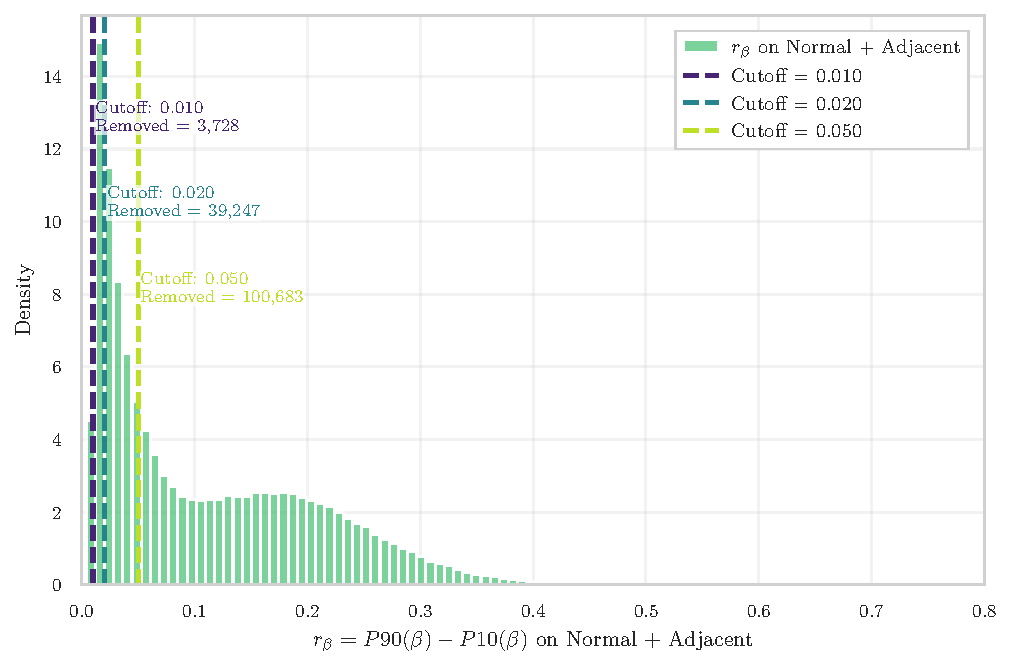
\includegraphics[width=\textwidth]{Figures/GSE69914_r_beta_distribution_NA_study_1.pdf}
        \caption{\(r_\beta\) distribution on Normal+Adjacent samples, with thresholds
        at 0.01, 0.02, and 0.05.}
    \end{subfigure}
    \hfill
    \begin{subfigure}[t]{0.49\textwidth}
        \centering
        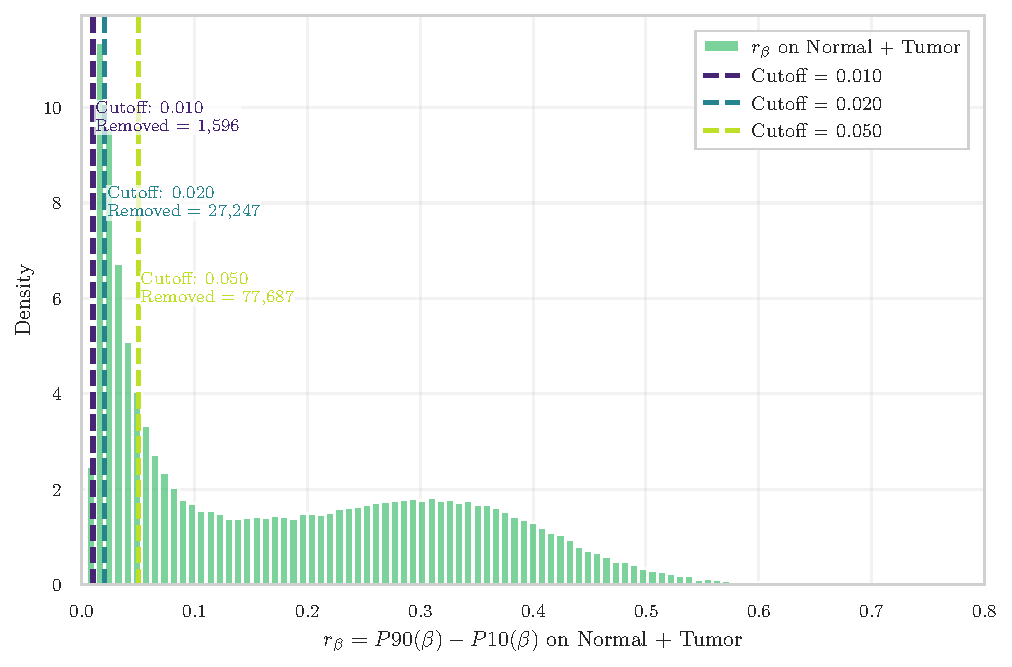
\includegraphics[width=\textwidth]{Figures/GSE69914_r_beta_distribution_NT_study_1.pdf}
        \caption{\(r_\beta\) distribution on Normal+Tumor samples.}
    \end{subfigure}
    \caption{\textbf{Variability range analysis (Edgar-style)}.  
    The Normal+Adjacent subset displays a large block of CpGs with extremely low
    variability (\(r_\beta < 0.05\)), supporting the use of invariance filtering
    to reduce biologically uninformative loci.}
    \label{fig:gse69914_rbeta_distributions}
\end{figure}

To assess whether variability patterns in N+A were consistent with N+T, a
scatter comparison between \(r_\beta^{(NA)}\) and \(r_\beta^{(NT)}\) was
generated (Fig.~\ref{fig:gse69914_variability_scatter}).  
The two measures exhibited strong concordance
(\good{Spearman~\(\rho = 0.845\)}), although a clear band of CpGs deviated
from the diagonal, corresponding precisely to the \textbf{breakdown loci}
defined above.

Further annotation-based analysis showed that invariants are not uniformly
distributed across genomic elements.
Invariant CpGs were enriched in promoter-proximal regions—particularly
\texttt{TSS200} and \texttt{1stExon}—while gene bodies and 3'UTRs were
underrepresented (Fig.~\ref{fig:gse69914_invariant_enrichment}).
This pattern mirrors the findings of Edgar~et~al.~\cite{Edgar2017}, who
reported that invariant CpGs preferentially occupy regulatory elements with
constitutively stable methylation profiles.

\begin{figure}[t]
    \centering
    % Left: scatter
    \begin{subfigure}[t]{0.49\textwidth}
        \centering
        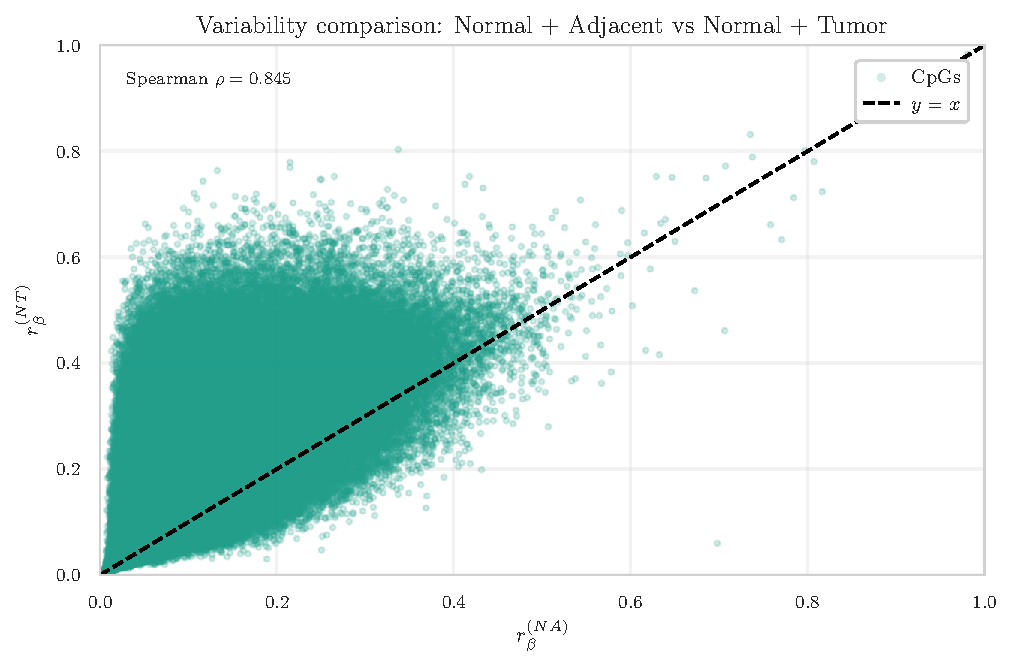
\includegraphics[width=\textwidth]{Figures/GSE69914_plot_scatter_rbeta_NA_vs_NT.pdf}
        \caption{Comparison of CpG variability between N+A and N+T.  
        Breakdown loci diverge from the identity line.}
    \end{subfigure}
    \hfill
    % Right: barplot enrichment
    \begin{subfigure}[t]{0.49\textwidth}
        \centering
        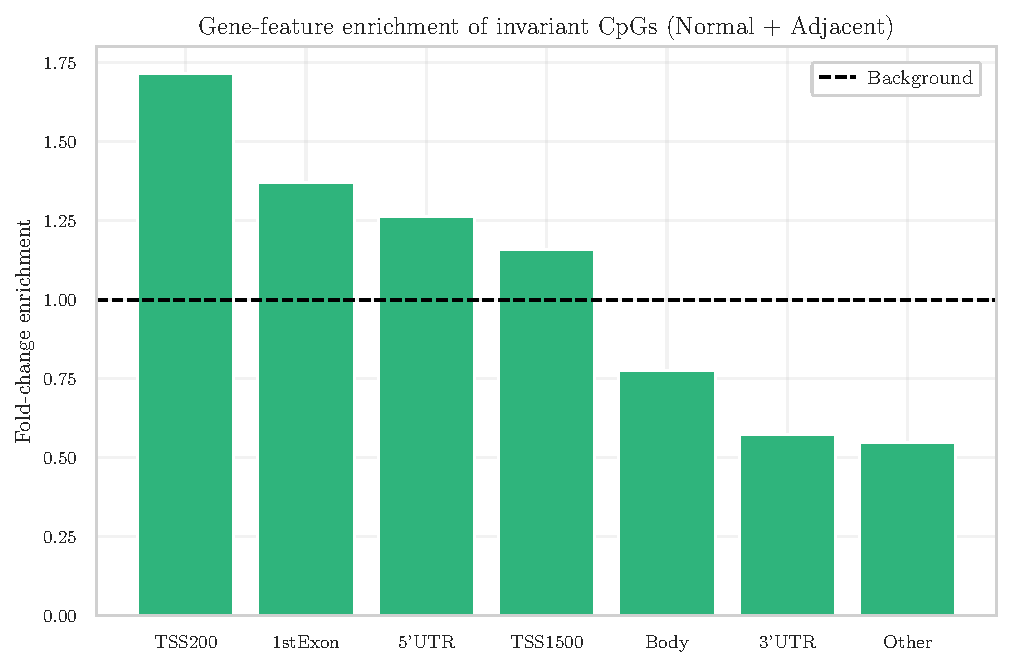
\includegraphics[width=\textwidth]{Figures/GSE69914_plot_enrichment_gene_invariant.pdf}
        \caption{Genomic enrichment of invariant N+A CpGs across gene features.}
        \label{fig:gse69914_invariant_enrichment}
    \end{subfigure}
    \caption{
        \textbf{Variability concordance and genomic context of invariant CpGs}.  
        Stable loci dominate the diagonal, while breakdown loci reflect tumour-induced
        methylation variability. Promoter regions show the strongest enrichment of
        invariant CpGs.}
    \label{fig:gse69914_variability_scatter}
\end{figure}

Invariants in breast tissue were compared with the three tissue
invariance sets published by Edgar~et~al.\ (blood, buccal, placenta).
Their intersection yielded \good{42{,}315 universal CpGs} shared across all
tissues.  
Among these, \good{30{,}251} remained invariant in Normal+Adjacent breast,
and \good{28{,}351} remained invariant even after including tumour samples.
A biologically relevant subset of \good{2{,}010 CpGs} belonged to the breakdown
category, suggesting possible tissue-specific loss of epigenetic stability in
tumourigenesis.

\begin{figure}[t]
    \centering
    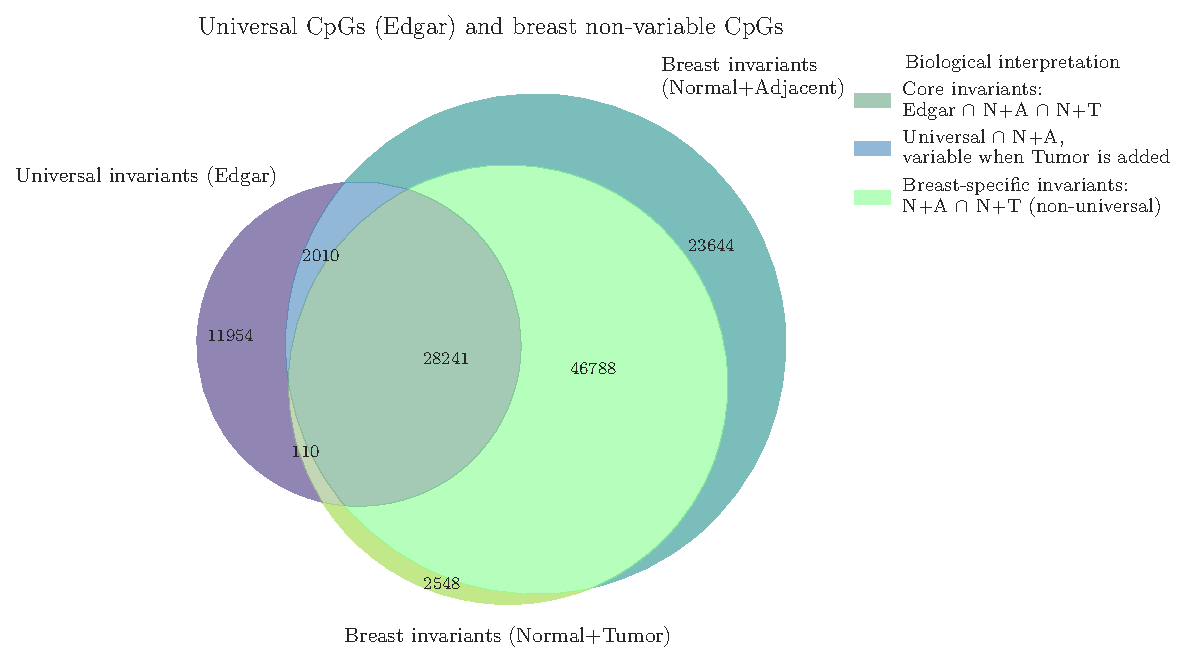
\includegraphics[width=0.72\textwidth]{Figures/GSE69914_venn_universal_vs_NA_vs_NT.pdf}
    \caption{
        \textbf{Intersection between universal invariant CpGs (Edgar) and breast invariants}.  
        Core invariants (Edgar~\(\cap\)~N+A~\(\cap\)~N+T) represent strongly conserved loci,
        whereas “breakdown loci’’ highlight CpGs losing stability specifically in tumour
        tissue.}
    \label{fig:gse69914_edgar_comparison}
\end{figure}

\paragraph{Step~4 -- $\beta$ to $M$ Conversion}
\label{par:gse69914_step4}

Illumina Infinium methylation arrays measure methylated ($y^{(M)}$) and unmethylated ($y^{(U)}$) signal intensities per CpG. 
The processed dataset provides only $\beta$-values,
\[
\beta = \frac{y^{(M)}}{y^{(M)} + y^{(U)}},
\]
a bounded proportion in $[0,1]$ characterised by strong mean–variance dependence. 
Following the foundational analysis of Du~\textit{et al.}~\cite{Du2010}, all $\beta$-values were transformed into $M$-values using the logit relation
\[
M = \log_2\!\left(\frac{\beta + \varepsilon}{1 - \beta + \varepsilon}\right),
\qquad \varepsilon = 10^{-6},
\]
which yields an approximately homoscedastic scale more suitable for linear modelling, empirical Bayes moderation, ComBat batch correction, and regression-based inference.

Importantly, the adoption of $M$-values is not only theoretically motivated but also widely implemented in practice.  
Several high-impact studies routinely perform statistical modelling in $M$-space while retaining $\beta$-values solely for biological interpretation and effect-size visualisation.  
Examples include the differential methylation analysis of purified human blood cell types by Reinius~\textit{et al.}~\cite{Reinius2012}, the methodological framework underlying the \texttt{minfi} pipeline described by Triche~\textit{et al.}~\cite{Triche2013}, and oncological applications such as the tumour hypoxia study by Thienpont~\textit{et al.}~\cite{Thienpont2016}, where all $\beta$-values were explicitly transformed to $M$-values prior to statistical testing.  
These examples illustrate that $M$-values have become a de facto standard for inferential analyses in Illumina 450K/EPIC workflows.

The conversion was applied to the complete post-filtering matrix (\good{150{,}800 CpGs} across \good{397 samples}).  
A manual inspection of transformed values confirmed correct numerical behaviour across the full CpG panel, including loci with extreme $\beta$ close to 0 or 1.

\noindent\textbf{Distributional consequences of the transformation.}
Fig.~\ref{fig:hist_msd_beta_m} illustrates in detail how the $\beta \rightarrow M$ mapping reshapes the empirical distribution of methylation.  
Normal and Adjacent tissues display the expected U-shaped profiles in $\beta$-space, reflecting biological accumulation near fully unmethylated or fully methylated states.  
After logit transformation, the corresponding $M$-value distributions become substantially more symmetric and comparable across groups, indicating that the transformation regularises the scale without distorting biological structure.

The mean–SD relationships further highlight this effect.  
In $\beta$-space, variance is strongly mean-dependent and inflates near the boundaries, whereas $M$-values exhibit markedly flatter SD profiles.  
This variance-stabilising behaviour is consistent with the theoretical findings of Du~\textit{et al.}~\cite{Du2010} and with the practical motivations underlying the adoption of $M$-values in modern methylation studies.

% ============================================================
% FIGURES: HISTOGRAMS + MEAN–SD FOR BETA AND M
% ============================================================
\begin{figure}[t]
    \centering

    % ---------------- ROW 1: HISTOGRAMS (Beta, Normal & Adjacent) ----------------
    \begin{subfigure}{0.24\textwidth}
        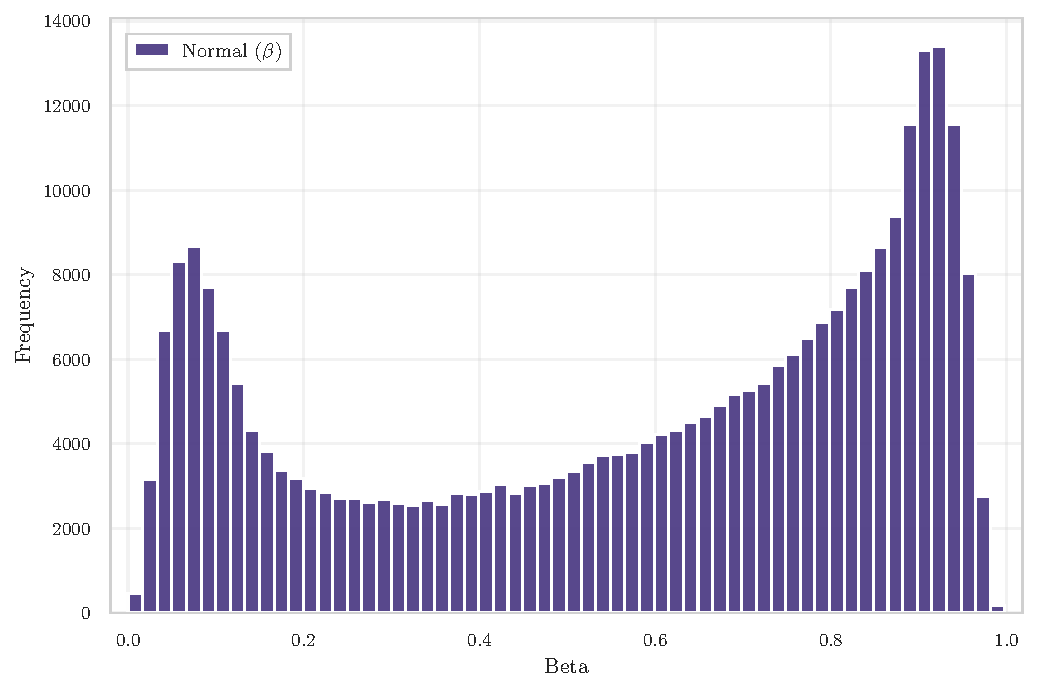
\includegraphics[width=\textwidth]{Figures/GSE69914_hist_normal_beta.pdf}
        \caption{Normal ($\beta$)}
    \end{subfigure}
    \begin{subfigure}{0.24\textwidth}
        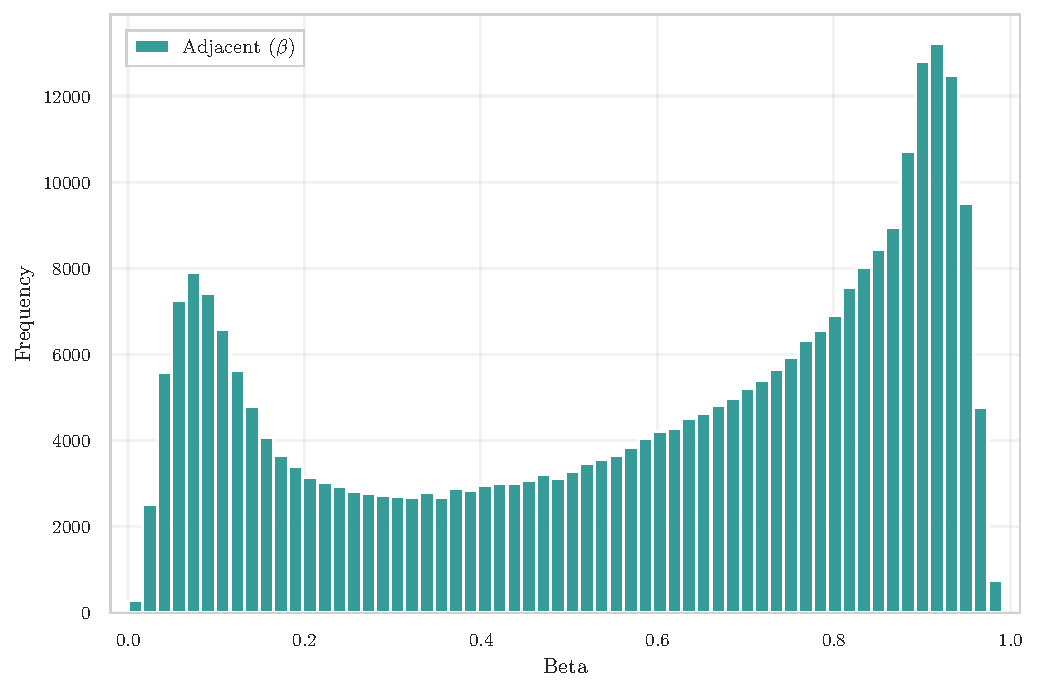
\includegraphics[width=\textwidth]{Figures/GSE69914_hist_adjacent_beta.pdf}
        \caption{Adjacent ($\beta$)}
    \end{subfigure}
    \begin{subfigure}{0.24\textwidth}
        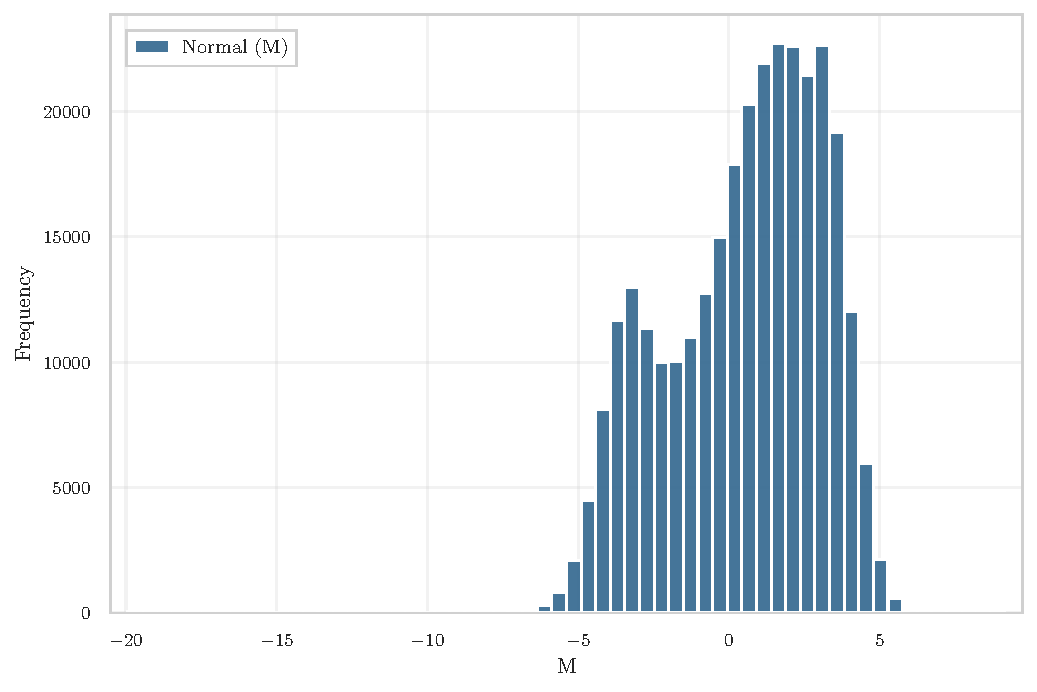
\includegraphics[width=\textwidth]{Figures/GSE69914_hist_normal_m.pdf}
        \caption{Normal ($M$)}
    \end{subfigure}
    \begin{subfigure}{0.24\textwidth}
        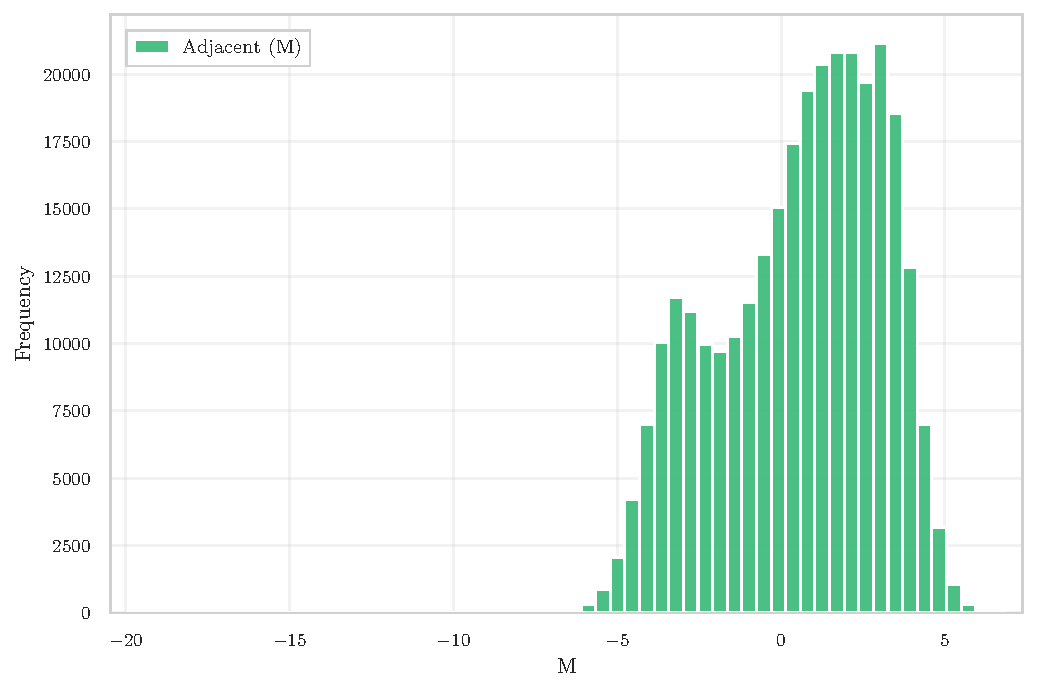
\includegraphics[width=\textwidth]{Figures/GSE69914_hist_adjacent_m.pdf}
        \caption{Adjacent ($M$)}
    \end{subfigure}

    \vspace{0.8em}

    % ---------------- ROW 2: MEAN–SD RELATIONS ----------------
    \begin{subfigure}{0.24\textwidth}
        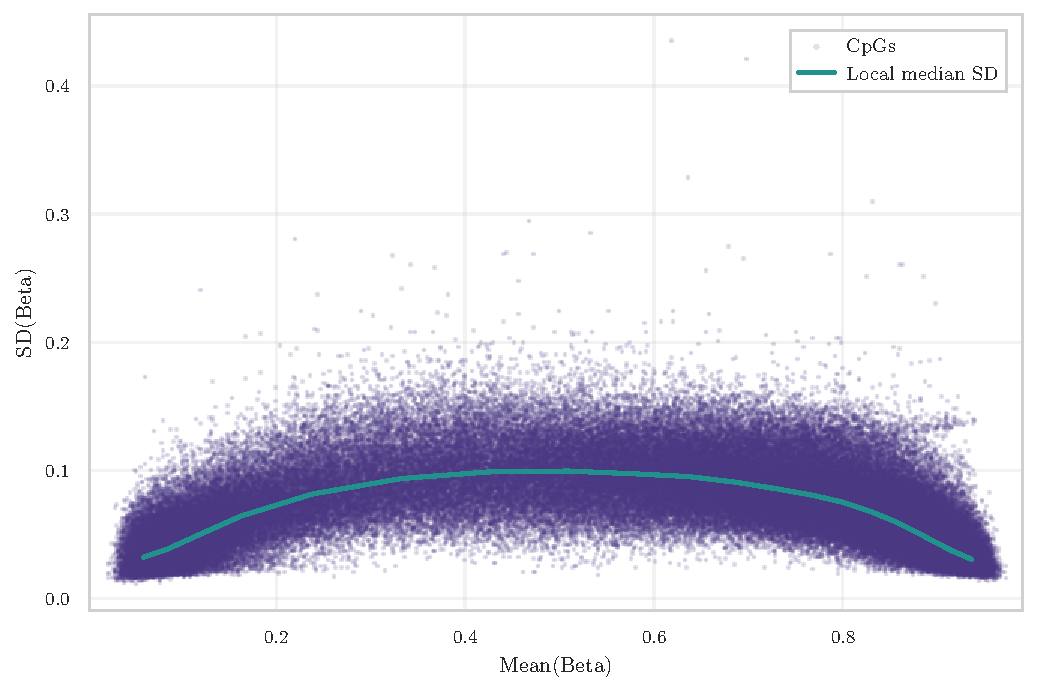
\includegraphics[width=\textwidth]{Figures/GSE69914_msd_normal_beta.pdf}
        \caption{Mean–SD Normal ($\beta$)}
    \end{subfigure}
    \begin{subfigure}{0.24\textwidth}
        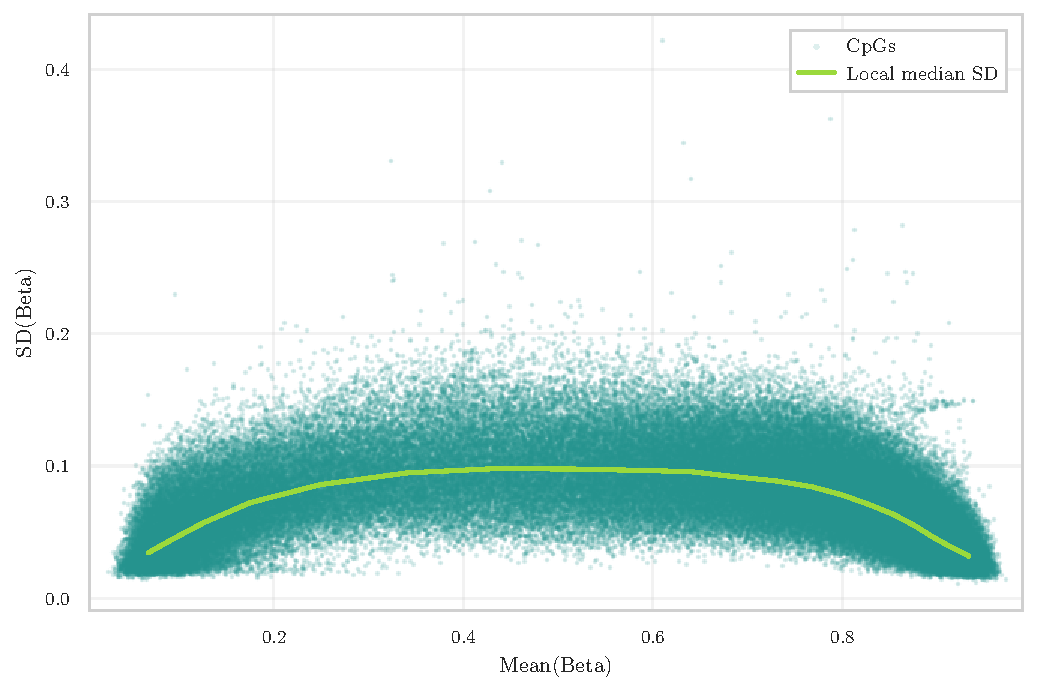
\includegraphics[width=\textwidth]{Figures/GSE69914_msd_adjacent_beta.pdf}
        \caption{Mean–SD Adjacent ($\beta$)}
    \end{subfigure}
    \begin{subfigure}{0.24\textwidth}
        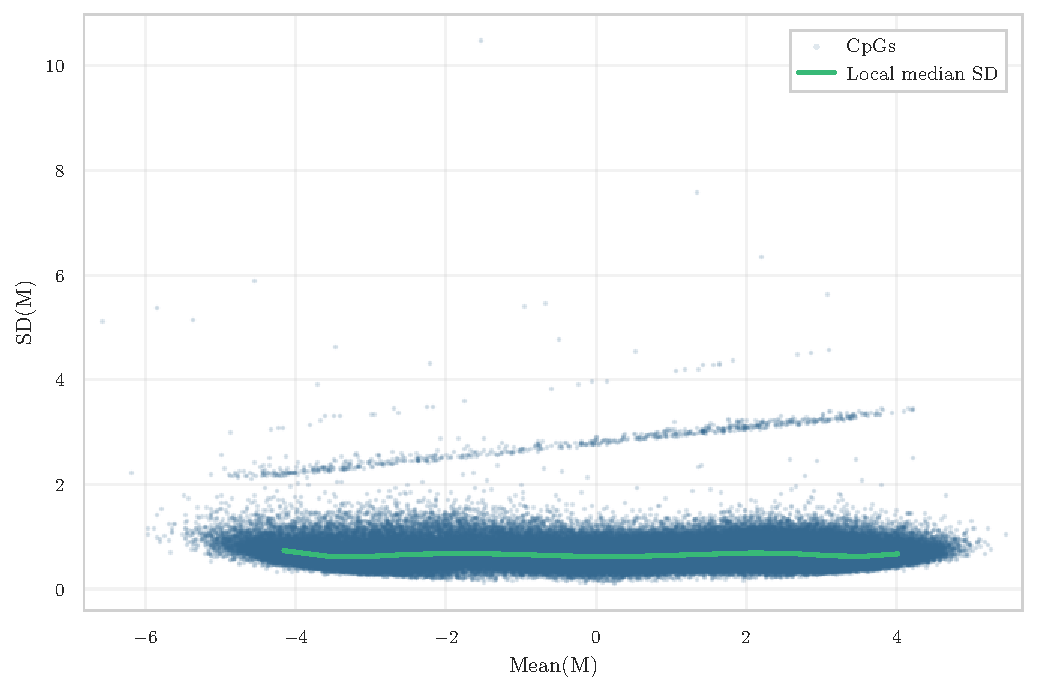
\includegraphics[width=\textwidth]{Figures/GSE69914_msd_normal_m.pdf}
        \caption{Mean–SD Normal ($M$)}
    \end{subfigure}
    \begin{subfigure}{0.24\textwidth}
        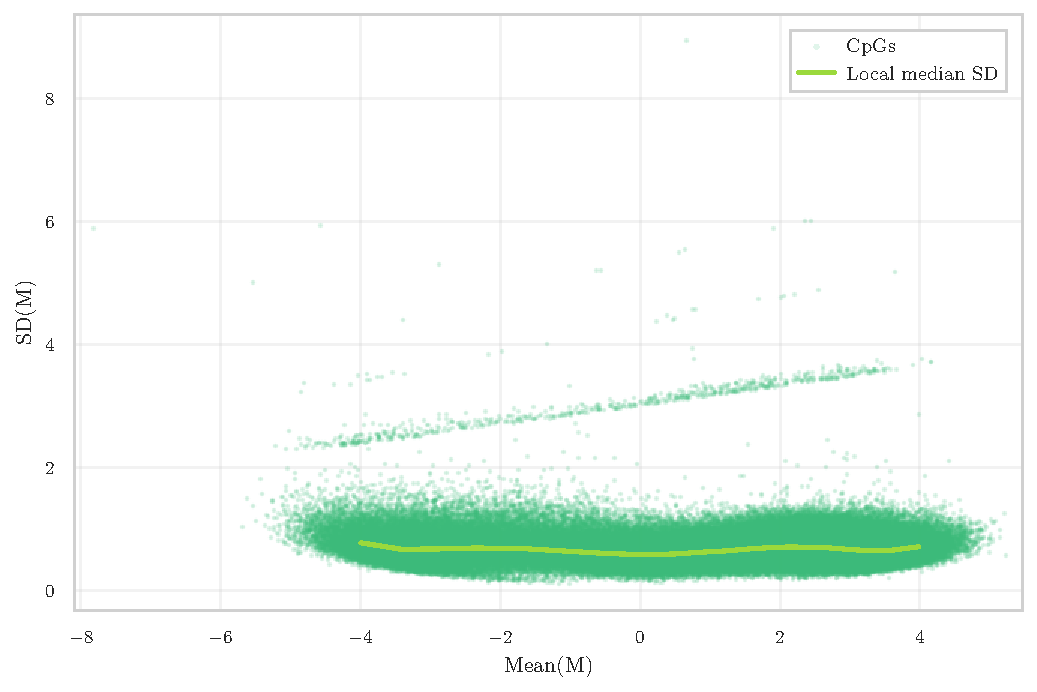
\includegraphics[width=\textwidth]{Figures/GSE69914_msd_adjacent_m.pdf}
        \caption{Mean–SD Adjacent ($M$)}
    \end{subfigure}

    \caption{
        \textbf{Distributional comparison between $\beta$ and $M$ quantifications in Normal and Normal-adjacent tissues.}  
        Top row: $\beta$ exhibits a bounded, U-shaped distribution, whereas $M$ shows an approximately symmetric profile.  
        Bottom row: The substantial mean-dependent variance in $\beta$ is dramatically reduced after transformation, confirming that $M$-values provide a more homoscedastic scale for statistical modeling.  
        All panels computed on the working set of \good{150{,}800 CpGs} after complete technical and invariance filtering.
    }
    \label{fig:hist_msd_beta_m}
\end{figure}


\paragraph{Step~5 -- Batch Effect Correction}
\label{par:gse69914_step3}

\paragraph{Step~6 -- Final Outputs}
\label{par:gse69914_step5}


% ============================================================
\subsection{Dataset GSE225845}
\label{subsec:gse225845_preproc}
% ============================================================

\paragraph{Step 0 — Initial Pre-processing}
\label{par:gse225845_step0}

\paragraph{Step 1 — Bias}
\label{par:gse225845_step0}

\paragraph{Step 1 — Technical Filtering}
\label{par:gse225845_step1}

\paragraph{Step 4 — Invariance Filtering on Normal+Adjacent}
\label{par:gse225845_step4}


\paragraph{Step 2 — $\beta$-to-$M$ Conversion}
\label{par:gse225845_step2}


\paragraph{Step 3 — Batch Effect Correction}
\label{par:gse225845_step3}




\paragraph{Step 5 — Final Outputs}
\label{par:gse225845_step5}



% ============================================================
\subsection{Dataset GSE287331}
\label{subsec:gse287331_preproc}
% ============================================================

\paragraph{Step 0 — Initial Pre-processing}
\label{par:gse287331_step0}

\subparagraph{Ingestion and Alignment}
\label{subpar:gse287331_ingestion}

\subparagraph{Coarse NaN Assessment}
\label{subpar:gse287331_nan}

\subparagraph{Infinium Type I/II Bias Diagnostics}
\label{subpar:gse287331_typebias}


\paragraph{Step 1 — Technical Filtering}
\label{par:gse287331_step1}

\subparagraph{Cross-reactive Probes}
\label{subpar:gse287331_chen_pidsley}

\subparagraph{EPIC Unreliable Probes}
\label{subpar:gse287331_mccartney}

\subparagraph{SNP-affected Probes}
\label{subpar:gse287331_snp}

\subparagraph{Non-CpG Probes}
\label{subpar:gse287331_noncpg}

\subparagraph{Sex-chromosome Probes}
\label{subpar:gse287331_xy}

\subparagraph{Technical Filtering Summary}
\label{subpar:gse287331_filter_summary}


\paragraph{Step 2 — $\beta$-to-$M$ Conversion}
\label{par:gse287331_step2}

\subparagraph{Definition of $\beta_{\text{clean}}$}
\label{subpar:gse287331_bclean}

\subparagraph{Logit Transformation}
\label{subpar:gse287331_mvalues}

\subparagraph{Usage of $\beta$ and M-values}
\label{subpar:gse287331_use_beta_m}


\paragraph{Step 3 — Batch Effect Correction}
\label{par:gse287331_step3}

\subparagraph{Pre-batch Diagnostics}
\label{subpar:gse287331_prebatch}

\subparagraph{Batch Model}
\label{subpar:gse287331_batchmodel}

\subparagraph{ComBat Application}
\label{subpar:gse287331_combat}

\subparagraph{Post-batch Verification}
\label{subpar:gse287331_postbatch}


\paragraph{Step 4 — Invariance Filtering on Normal+Adjacent}
\label{par:gse287331_step4}

\subparagraph{NA Subset Selection}
\label{subpar:gse287331_na_subset}

\subparagraph{Variability Metrics}
\label{subpar:gse287331_variability}

\subparagraph{Threshold Selection}
\label{subpar:gse287331_threshold}

\subparagraph{Creation of Final Mask}
\label{subpar:gse287331_mask}


\paragraph{Step 5 — Final Outputs}
\label{par:gse287331_step5}

\subparagraph{Final Matrices}
\label{subpar:gse287331_final_matrices}

\subparagraph{CpG Tracking}
\label{subpar:gse287331_tracking}

\subparagraph{Mini-report Summary (optional)}
\label{subpar:gse287331_minireport}



% ============================================================
\section{Inter-Dataset Analysis}
\label{sec:inter_dataset}

% (intentionally left empty)



\section{Data Validation and Integrity Check}\label{sec:data_validation}



\paragraph{Missing Value Analysis.}
Next, I performed a comprehensive check for missing values ($\text{NaN}$), as these can severely impact model performance and must be addressed before training.

\begin{itemize}[label=-]
    \item No missing entries ($\text{NaN}$) were detected across any CpG probe.
    \good{Total NaN count: 0 |  Overall missing rate: 0\%.}
    
    \item The methylation matrix is therefore \textbf{complete}, requiring \textbf{no filtering or imputation} procedures.
    \good{Dataset confirmed fully complete.}
    
    \item For future datasets:
    \begin{itemize}[label=--]
        \item If the overall missing rate is $< 1\%$, imputation may be considered as an optional step.
        \item If probe missingness exceeds $5\%$ or sample missingness exceeds $10\%$, the affected entities should be discarded, following standard preprocessing practices~\cite{zhou2016}.
    \end{itemize}
\end{itemize}


This validation confirms the dataset is structurally sound, numerically consistent, and complete, enabling unbiased downstream variance modeling, differential methylation testing, and batch correction without any further cleaning.















\clearpage

\appendix
\section{Filtering lists}
\label{app:probe-filters}

This appendix details the major technical filtering lists and annotations applied in Illumina 450K and EPIC methylation arrays to remove unreliable or ambiguous CpG probes. 

\begin{table}[H]
\small
\caption{Technical categories covered by each filtering resource.}
\centerline{ % <-- USA QUESTO
\begin{tabular}{lccccc}
\toprule
\textbf{Category} & \textbf{Naeem} \ref{app:naeem2014} & \textbf{Chen} \ref{app:chen2013} & \textbf{Pidsley} \ref{app:pidsley2016} & \textbf{Zhou} \ref{app:zhou2016} & \textbf{McCartney} \ref{app:mccartney2016}\\
\midrule
Cross-hybridisation / multi-mapping & Yes (Steps 1–2) & Yes & Yes & \texttt{MASK\_mapping} & Table~2+3 \\
SNP at CpG / extension base   	& Yes (Step 5) & -- & Yes & \texttt{MASK\_snp5, MASK\_extBase} & -- \\
Nearby SNP tolerated   	& Conditional (Step 6) & -- & -- & -- & -- \\
INDEL / structural variant   	& Yes (Step 3) & -- & -- & -- & -- \\
Non-CpG probes   	& -- & -- & Yes 	& \texttt{MASK\_nonCG} & Table~3 \\

\bottomrule
\end{tabular}
} 
\end{table}

\subsection{Reducing the risk of false discovery enabling identification of biologically significant genome-wide methylation status using the humanmethylation450 array}
\label{app:naeem2014}
\begin{wrapfigure}{r}{0.29\textwidth} % {r}=destra, {0.4\textwidth}=larghezza
    \centering
    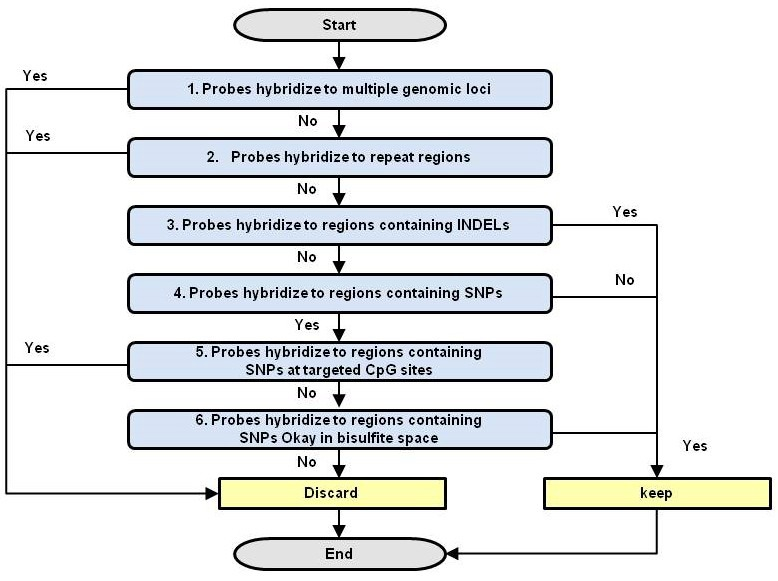
\includegraphics[width=\linewidth]{Figures/Workflow for determining affected Probes.jpg} % o .png, .pdf, .eps...
    \caption{Workflow for determining affected Probes.}
    \label{fig:Workflow}
\end{wrapfigure}
Naeem \emph{et al.} \cite{naeem2014} proposed a structured filtering framework to reduce false discoveries by sequentially discarding probes based on hybridisation specificity and genomic integrity (Figure \ref{fig:Workflow}).  
The main exclusion steps are:
\begin{enumerate}[label=-]
  \item Multi-mapping or cross-hybridising probes $\Rightarrow$ \textit{discard}.
  \item Probes overlapping repetitive elements (LINE/SINE/ALU) $\Rightarrow$ \textit{discard}.
  \item Probes targeting regions with INDELs $\Rightarrow$ \textit{discard}.
  \item Probes overlapping SNPs:
    \begin{enumerate}[label=--]
      \item SNP at CpG or extension site $\Rightarrow$ \textit{discard}.
      \item SNP near target but not interfering in bisulfite space $\Rightarrow$ \textit{keep}.
    \end{enumerate}
\end{enumerate}
The resulting ``discard'' set therefore removes probes affected by cross-reactivity, structural polymorphisms (INDELs), and SNPs that alter CpG interrogation.

\subsection{Discovery of cross-reactive probes and polymorphic cpgs in the illumina infinium humanmethylation450 microarray}
\label{app:chen2013}
Chen \emph{et al.} \cite{chen2013} empirically identified probes in the 450K array that exhibit off-target hybridisation or overlap with common SNPs.  
For this project, only the \textbf{cross-reactive list} is available and used.  
This list enumerates $\sim$29k multi-mapping probes whose methylation signal cannot be uniquely attributed to one genomic locus.

\subsection{Critical evaluation of the Illumina MethylationEPIC BeadChip microarray for whole-genome DNA methylation profiling}
\label{app:pidsley2016}
Pidsley \emph{et al.} \cite{pidsley2016} provide a platform-level assessment of the EPIC array, with explicit \emph{annotated probe lists} that flag probes whose methylation signal may be confounded by design- or genome-related artefacts. The focus is on probe categories and positions where technical bias arises, rather than on a universal, prescriptive blacklist. In particular, they catalogue:

\begin{itemize}[label=-]
  \item \textbf{Cross-hybridising CpG-targeting probes:} CpG probes showing sequence homology (off-target matches) to additional genomic loci, yielding non-unique hybridisation and potentially inflated or ambiguous $\beta$ signals.
  \item \textbf{Cross-hybridising non-CpG-targeting probes:} off-target issues among CNG/non-CpG probes; these are typically excluded in CpG-centric analyses due to limited interpretability and higher risk of artefacts.
  \item \textbf{Probes overlapping common genetic variation:} annotation of variants from population data at three critical positions:
  \begin{enumerate}[label=--]
    \item \textit{At the interrogated CpG} (polymorphic CpG) --- directly affects the presence of the CpG dinucleotide and the measured methylation state;
    \item \textit{At the single-base extension (SBE) site} (Type~I) --- perturbs extension and dye chemistry, biasing intensity ratios;
    \item \textit{Within the probe body} --- can reduce binding affinity or alter hybridisation kinetics, especially for common variants.
  \end{enumerate}
\end{itemize}


\subsection{Comprehensive characterization, annotation and innovative use of infinium dna methylation beadchip probes}
\label{app:zhou2016}
Zhou \emph{et al.} \cite{zhou2016} released a unified probe annotation for both 450K and EPIC arrays with multiple binary mask columns (\texttt{MASK\_*}).  
Each \href{https://zwdzwd.github.io/InfiniumAnnotation/mask.html}{mask} flags probes to be removed due to specific technical artifacts.
\begin{itemize}[label=-]
  \item \texttt{MASK.mapping}: probes with low or inconsistent mapping quality (non-unique alignment or presence of INDELs);
  \item \texttt{MASK.typeINextBaseSwitch}: Type-I probes carrying a SNP in the extension base that causes a color-channel switch (\emph{CCS} probes);
  \item \texttt{MASK.extBase}: probes whose extension base is inconsistent with the expected color channel or CpG context;
  \item \texttt{MASK.sub30.copy}: probes with non-unique 30-bp 3' subsequences (potential cross-hybridisation);
  \item \texttt{MASK.snp5.common}: probes overlapping a SNP within $\pm5$\,bp of the interrogated CpG (even with global MAF < 1\%);
  \item \texttt{MASK.snp5.GMAF1p}: probes overlapping SNPs with global MAF > 1\%;
  \item \texttt{MASK.general}: recommended composite mask integrating mapping, SNP, and cross-reactivity filters for general use;
  \item \texttt{MASK.rmsk15}: probes overlapping RepeatMasker regions (not recommended for exclusion in standard workflows).
\end{itemize}

This resource provides a programmatic and reproducible way to perform fine-grained probe masking.

\subsection{Identification of polymorphic and off-target probe binding sites on the Illumina Infinium MethylationEPIC BeadChip}
\label{app:mccartney2016}
McCartney \emph{et al.} \cite{mccartney2016} assessed probe design artifacts and published supplementary tables that include:
\begin{itemize}[label=-]
  \item Cross-hybridising CpG-targeting probes;
  \item Cross-hybridising non-CpG-targeting probes.
\end{itemize}



\printbibliography
\end{document}
